\documentclass{article}
\usepackage{iclr2016_conference,times}

\usepackage{subfig}
\usepackage{float}
\usepackage{hyperref}
\usepackage{url}
\usepackage{amsmath,amssymb}
\usepackage{natbib}
\usepackage{wrapfig}
\usepackage{graphicx}
\bibliographystyle{abbrvnat}

\title{
	Mobile Computing (CS23400$/$1) \vspace{-4pt} \\
	{\Large Lab 1 - Report} \vspace{6pt} \\
	{\large Andrea F. Daniele $\hspace{2.2cm}$ Max X. Liu $\hspace{2.2cm}$ Noah A. Hirsch}
}

\begin{document}

\maketitle


\vspace{-1.2cm}

\section{Task}
\vspace{-.3cm}
The goal of this lab is to collect and leverage IMU data from a small robotic
car to classify a set of activities. Using the IMU data we can implement machine
learning models to classify IMU traces into four distinct activities (walking,
jumping, standing, driving). Furthermore, the classification model used should
be robust to challenges with low quality IMU's and mobile computation limits.

\section{Challenges}
\vspace{-.3cm}
One of the primary challenges faced was extracting consistent and relevant data
from the IMU traces. Due to imperfect measurements from the IMU, the raw data
contains a lot of noisy readings that complicate the problem of classifying
activities. Furthermore, it is very computationally intensive to train Recurrent
Neural Networks with such large trace files; additional pre-processing of data
is necessary to help train the model. An additional concern was that there may
not be enough data and/or features to effectively train a Recurrent Neural Network.

\section{Proposed Approach}
\vspace{-.3cm}
\textbf{Assigned to: Max}

The task naturally lended itself to a general data classification problem. We decided
to use a Recurrent Neural Network to solve this problem; specifically, we used LSTM
(Long Short Term Memory) networks. RNN's are extremely effective with this type of
trace data because it is able to take in sequences of data and make classifications
based on the context of both recent and past information. Thus, we can easily look at features
such as changes in x, y, z acceleration over some period of time. In order to quickly and effectively train
the RNN it is necessary to first do some data processing to reduce noise, decrease trace sizes, and
add additional features.


* Let's introduce the fact that we do some data post-processing before feeding it to the model
(the next section will be about data post-processing).

\subsection{Data post-processing}
\vspace{-.3cm}
\textbf{Assigned to: Andrea}

* Here we talk about the fact that we downsample the readings from $128Hz$ to $16Hz$. Let's
justify it by saying that we tried different factors and empirically chose the one that maximizes
reduction while preserving signal shape (we tried $2, 4, 8, 16, 32$).

* Let's also talk about the trimming phase, in which we discard the first and last $2$ seconds
of each trace because of the time spent to say ''Now you can start jumping``, or the time
required to switch windows (while Driving the car) and the time when somebody stops earlier and
asks ''Can I stop jumping?``.

* We also explain that since the signals are periodic (for all the activities that we have), we can
easily classify the activity based on a few seconds of data. Thus we split a $10$ seconds long
trace into $6$ smaller samples of $1$ second each (the $4$ seconds that are missing are removed
in the trimming phase above).


\subsection{Recurrent Neural Network}
\vspace{-.3cm}
\textbf{Assigned to: Andrea}

* Here we explain and show the architecture of our neural network by unwrapping the timesteps.

* Explain what is X, what is Y, and what is the hidden state. Do not talk about batching here.

* Explain (briefly) the training process and how gradient back-propagation works.


\subsection{Dataset}
\vspace{-.3cm}
\textbf{Assigned to: Andrea}

* Here we just talk about how much data (samples) we used for training, how much for validation
and how much for testing.

* Depending on whether we decide to use cross-validation we talk about it too.


\section{Results}
\vspace{-.3cm}
\textbf{Assigned to: Noah}

\t The accuracy of our recurrent neural network is very high. Having cut each trace into one-second samples, each epoch of training contained 1041 samples. After only 4 epochs of training, our training accuracy hit 100\% as well as our post-epoch testing accuracy. Of course, this varied throughout the 50-epoch training, but accuracy remained near-perfect through all epochs after 3. The inclusion of the first derivative of acceleration with respect to time raised the accuracy of our model by almost 25\%, as it allowed the RNN to access the shape of the acceleration readings. Included below in Figure 1 is a plot of per-trace accuracy over the 50 epochs, which shows the rate of cross-validation correctness for each epoch.

\begin{figure}[h]
    \centering
    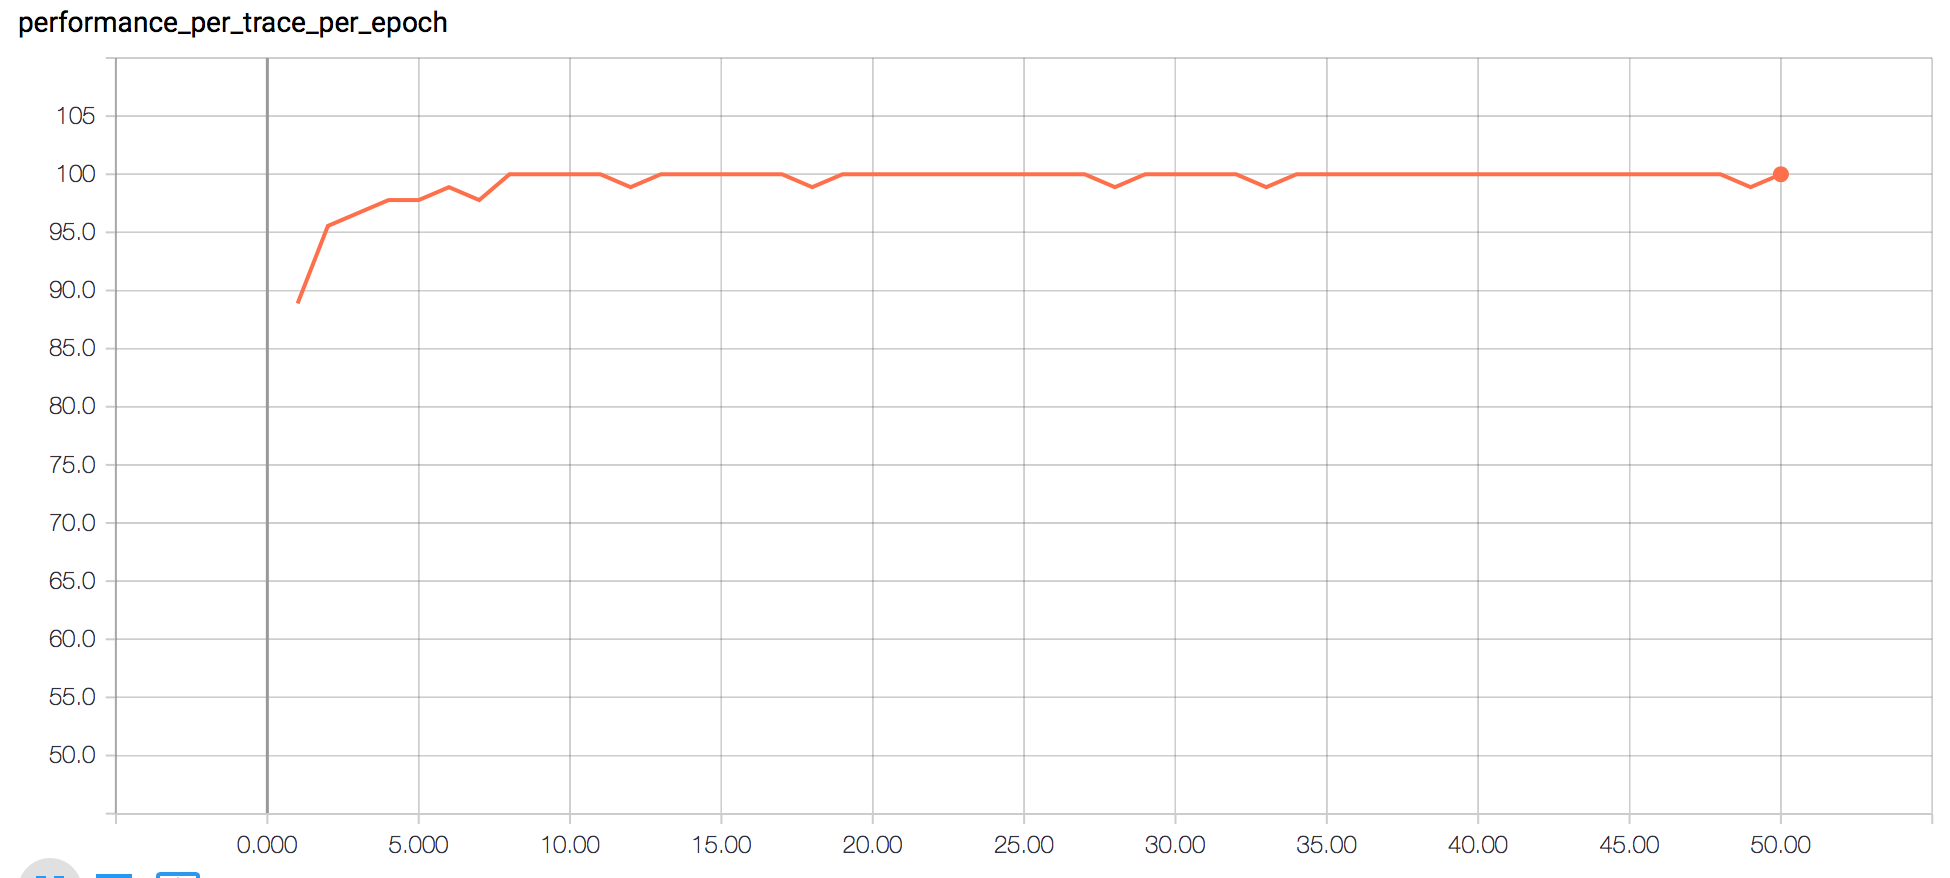
\includegraphics[width=0.7\linewidth]{figures/acc_ptpe.png}
    \caption{Accuracy per-trace per-epoch \label{fig:acc_ptpe}}
\end{figure}

\t Using held-out data, which is data that was not included in any of the training epochs, we observe testing accuracy of about 92\%, which is very high. The accuracy reduction is due to the model having difficulty distinguishing between standing and walking. We anticipate with more time and traces, this confusion will decrease as the model learns the subtle distinctions between the two activites. Shown below in Figure 2 is the corresponding confusion matrix for the final epoch using held-out data.

\begin{figure}[h]
    \centering
    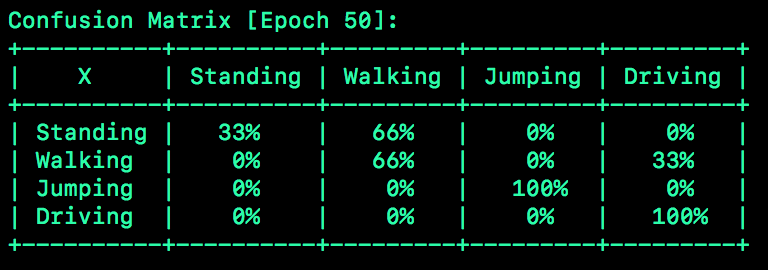
\includegraphics[width=0.8\linewidth]{figures/confusion.png}
    \caption{Confusion Matrix \label{fig:confusion}}
\end{figure}

\section{Conclusion}
\vspace{-.3cm}
\textbf{Assigned to: Noah}

\t Overall, this algorithm is very promising. It only relies on the reading of a sensor that is very popular in mobile devices, the IMU. After training, it requires very low CPU and battery usage for activity identification, and can be easily run in the background on many devices. Additionally, there exists extensive implementation of tensorflow for a variety of mobile devices. So, this algorithm can be deployed easily and seamlessly to mobile devices whether on a vehicle or on a smartphone. Expansion of this model to include more realistic identification classes, such as turning, would allow one to achieve accurate activity detection for many uses concerning safety and usability.  


\end{document}
